\documentclass[a4wide]{article}

\usepackage{amsmath}
\usepackage{amstext, amsthm, amscd, bm, amsfonts, amssymb}
\usepackage{mathrsfs}
\usepackage{mathtools}
\usepackage{a4wide}
\usepackage{csquotes}
% \usepackage[english]{babel}
\usepackage[hidelinks]{hyperref}
\usepackage{cleveref}
\usepackage{nameref}
\usepackage[shortlabels]{enumitem}
\usepackage{faktor}
\usepackage{xcolor}
\usepackage{graphicx}
\usepackage{scrextend}
\usepackage{siunitx}
\usepackage{placeins}
\usepackage{caption}
\usepackage{subcaption}
\usepackage{algorithm}
\usepackage{algpseudocodex}

\usepackage[backend=bibtex, style=alphabetic]{biblatex}

\newcommand{\R}{\mathbb{R}}
\newcommand{\C}{\mathbb{C}}
\newcommand{\N}{\mathbb{N}}
\newcommand{\Z}{\mathbb{Z}}
\renewcommand{\P}{\mathbb{P}}
\newcommand{\ind}{\mathds{1}}

% blackboard letters
\providecommand{\bbA}{\mathbb{A}}
\providecommand{\bbB}{\mathbb{B}}
\providecommand{\bbC}{\mathbb{C}}
\providecommand{\bbD}{\mathbb{D}}
\providecommand{\bbE}{\mathbb{E}}
\providecommand{\bbF}{\mathbb{F}}
\providecommand{\bbG}{\mathbb{G}}
\providecommand{\bbH}{\mathbb{H}}
\providecommand{\bbI}{\mathbb{I}}
\providecommand{\bbJ}{\mathbb{J}}
\providecommand{\bbK}{\mathbb{K}}
\providecommand{\bbL}{\mathbb{L}}
\providecommand{\bbM}{\mathbb{M}}
\providecommand{\bbN}{\mathbb{N}}
\providecommand{\bbO}{\mathbb{O}}
\providecommand{\bbP}{\mathbb{P}}
\providecommand{\bbQ}{\mathbb{Q}}
\providecommand{\bbR}{\mathbb{R}}
\providecommand{\bbS}{\mathbb{S}}
\providecommand{\bbT}{\mathbb{T}}
\providecommand{\bbU}{\mathbb{U}}
\providecommand{\bbV}{\mathbb{V}}
\providecommand{\bbW}{\mathbb{W}}
\providecommand{\bbX}{\mathbb{X}}
\providecommand{\bbY}{\mathbb{Y}}
\providecommand{\bbZ}{\mathbb{Z}}

% calligraphic letters
\providecommand{\CA}{\mathcal{A}}
\providecommand{\CB}{\mathcal{B}}
\providecommand{\CC}{\mathcal{C}}
\providecommand{\CD}{\mathcal{D}}
\providecommand{\CE}{\mathcal{E}}
\providecommand{\CF}{\mathcal{F}}
\providecommand{\CG}{\mathcal{G}}
\providecommand{\CH}{\mathcal{H}}
\providecommand{\CI}{\mathcal{I}}
\providecommand{\CJ}{\mathcal{J}}
\providecommand{\CK}{\mathcal{K}}
\providecommand{\CL}{\mathcal{L}}
\providecommand{\CM}{\mathcal{M}}
\providecommand{\CN}{\mathcal{N}}
\providecommand{\CO}{\mathcal{O}}
\providecommand{\CP}{\mathcal{P}}
\providecommand{\CQ}{\mathcal{Q}}
\providecommand{\CR}{\mathcal{R}}
\providecommand{\CS}{\mathcal{S}}
\providecommand{\CT}{\mathcal{T}}
\providecommand{\CU}{\mathcal{U}}
\providecommand{\CV}{\mathcal{V}}
\providecommand{\CW}{\mathcal{W}}
\providecommand{\CX}{\mathcal{X}}
\providecommand{\CY}{\mathcal{Y}}
\providecommand{\CZ}{\mathcal{Z}}

% Capital bold characters in math mode
\providecommand{\BA}{{\boldsymbol{A}}}
\providecommand{\BB}{{\boldsymbol{B}}}
\providecommand{\BC}{{\boldsymbol{C}}}
\providecommand{\BD}{{\boldsymbol{D}}}
\providecommand{\BE}{{\boldsymbol{E}}}
\providecommand{\BF}{{\boldsymbol{F}}}
\providecommand{\BG}{{\boldsymbol{G}}}
\providecommand{\BH}{{\boldsymbol{H}}}
\providecommand{\BI}{{\boldsymbol{I}}}
\providecommand{\BJ}{{\boldsymbol{J}}}
\providecommand{\BK}{{\boldsymbol{K}}}
\providecommand{\BL}{{\boldsymbol{L}}}
\providecommand{\BM}{{\boldsymbol{M}}}
\providecommand{\BN}{{\boldsymbol{N}}}
\providecommand{\BO}{{\boldsymbol{O}}}
\providecommand{\BP}{{\boldsymbol{P}}}
\providecommand{\BQ}{{\boldsymbol{Q}}}
\providecommand{\BR}{{\boldsymbol{R}}}
\providecommand{\BS}{{\boldsymbol{S}}}
\providecommand{\BT}{{\boldsymbol{T}}}
\providecommand{\BU}{{\boldsymbol{U}}}
\providecommand{\BV}{{\boldsymbol{V}}}
\providecommand{\BW}{{\boldsymbol{W}}}
\providecommand{\BX}{{\boldsymbol{X}}}
\providecommand{\BY}{{\boldsymbol{Y}}}
\providecommand{\BZ}{{\boldsymbol{Z}}}

\providecommand{\Ba}{{\boldsymbol{a}}}
\providecommand{\Bb}{{\boldsymbol{b}}}
\providecommand{\Bc}{{\boldsymbol{c}}}
\providecommand{\Bd}{{\boldsymbol{d}}}
\providecommand{\Be}{{\boldsymbol{e}}}
\providecommand{\Bf}{{\boldsymbol{f}}}
\providecommand{\Bg}{{\boldsymbol{g}}}
\providecommand{\Bh}{{\boldsymbol{h}}}
\providecommand{\Bi}{{\boldsymbol{i}}}
\providecommand{\Bj}{{\boldsymbol{j}}}
\providecommand{\Bk}{{\boldsymbol{k}}}
\providecommand{\Bl}{{\boldsymbol{l}}}
\providecommand{\Bm}{{\boldsymbol{m}}}
\providecommand{\Bn}{{\boldsymbol{n}}}
\providecommand{\Bo}{{\boldsymbol{o}}}
\providecommand{\Bp}{{\boldsymbol{p}}}
\providecommand{\Bq}{{\boldsymbol{q}}}
\providecommand{\Br}{{\boldsymbol{r}}}
\providecommand{\Bs}{{\boldsymbol{s}}}
\providecommand{\Bt}{{\boldsymbol{t}}}
\providecommand{\Bu}{{\boldsymbol{u}}}
\providecommand{\Bv}{{\boldsymbol{v}}}
\providecommand{\Bw}{{\boldsymbol{w}}}
\providecommand{\Bx}{{\boldsymbol{x}}}
\providecommand{\By}{{\boldsymbol{y}}}
\providecommand{\Bz}{{\boldsymbol{z}}}

% bold upright letters for vectors
\newcommand{\VA}{{\mathbf{A}}}
\newcommand{\VB}{{\mathbf{B}}}
\newcommand{\VC}{{\mathbf{C}}}
\newcommand{\VD}{{\mathbf{D}}}
\newcommand{\VE}{{\mathbf{E}}}
\newcommand{\VF}{{\mathbf{F}}}
\newcommand{\VG}{{\mathbf{G}}}
\newcommand{\VH}{{\mathbf{H}}}
\newcommand{\VI}{{\mathbf{I}}}
\newcommand{\VJ}{{\mathbf{J}}}
\newcommand{\VK}{{\mathbf{K}}}
\newcommand{\VL}{{\mathbf{L}}}
\newcommand{\VM}{{\mathbf{M}}}
\newcommand{\VN}{{\mathbf{N}}}
\newcommand{\VO}{{\mathbf{O}}}
\newcommand{\VP}{{\mathbf{P}}}
\newcommand{\VQ}{{\mathbf{Q}}}
\newcommand{\VR}{{\mathbf{R}}}
\newcommand{\VS}{{\mathbf{S}}}
\newcommand{\VT}{{\mathbf{T}}}
\newcommand{\VU}{{\mathbf{U}}}
\newcommand{\VV}{{\mathbf{V}}}
\newcommand{\VW}{{\mathbf{W}}}
\newcommand{\VX}{{\mathbf{X}}}
\newcommand{\VY}{{\mathbf{Y}}}
\newcommand{\VZ}{{\mathbf{Z}}}

\newcommand{\Va}{{\mathbf{a}}}
\newcommand{\Vb}{{\mathbf{b}}}
\newcommand{\Vc}{{\mathbf{c}}}
\newcommand{\Vd}{{\mathbf{d}}}
\newcommand{\Ve}{{\mathbf{e}}}
\newcommand{\Vf}{{\mathbf{f}}}
\newcommand{\Vg}{{\mathbf{g}}}
\newcommand{\Vh}{{\mathbf{h}}}
\newcommand{\Vi}{{\mathbf{i}}}
\newcommand{\Vj}{{\mathbf{j}}}
\newcommand{\Vk}{{\mathbf{k}}}
\newcommand{\Vl}{{\mathbf{l}}}
\newcommand{\Vm}{{\mathbf{m}}}
\newcommand{\Vn}{{\mathbf{n}}}
\newcommand{\Vo}{{\mathbf{o}}}
\newcommand{\Vp}{{\mathbf{p}}}
\newcommand{\Vq}{{\mathbf{q}}}
\newcommand{\Vr}{{\mathbf{r}}}
\newcommand{\Vs}{{\mathbf{s}}}
\newcommand{\Vt}{{\mathbf{t}}}
\newcommand{\Vu}{{\mathbf{u}}}
\newcommand{\Vv}{{\mathbf{v}}}
\newcommand{\Vw}{{\mathbf{w}}}
\newcommand{\Vx}{{\mathbf{x}}}
\newcommand{\Vy}{{\mathbf{y}}}
\newcommand{\Vz}{{\mathbf{z}}}

\newcommand{\Vzero}{\boldsymbol{0}}

% Bold upright capital greek letters for _V_ectors and Matrices
\newcommand{\VGamma}  {\mathbf{\Gamma}}
\newcommand{\VDelta}  {\mathbf{\Delta}}
\newcommand{\VTheta}  {\mathbf{\Theta}}
\newcommand{\VLambda} {\mathbf{\Lambda}}
\newcommand{\VXi}     {\mathbf{\Xi}}
\newcommand{\VPi}     {\mathbf{\Pi}}
\newcommand{\VPsi}    {\mathbf{\Psi}}
\newcommand{\VSigma}  {\mathbf{\Sigma}}
\newcommand{\VUpsilon}{\mathbf{\Upsilon}}
\newcommand{\VPhi}    {\mathbf{\Phi}}
\newcommand{\VOmega}  {\mathbf{\Omega}}

% _B_old italicized capital greek letters
\newcommand{\BGamma}  {\boldsymbol{\mathit{\Gamma}}}
\newcommand{\BDelta}  {\boldsymbol{\mathit{\Delta}}}
\newcommand{\BTheta}  {\boldsymbol{\mathit{\Theta}}}
\newcommand{\BLambda} {\boldsymbol{\mathit{\Lambda}}}
\newcommand{\BXi}     {\boldsymbol{\mathit{\Xi}}}
\newcommand{\BPi}     {\boldsymbol{\mathit{\Pi}}}
\newcommand{\BPsi}    {\boldsymbol{\mathit{\Psi}}}
\newcommand{\BSigma}  {\boldsymbol{\mathit{\Sigma}}}
\newcommand{\BUpsilon}{\boldsymbol{\mathit{\Upsilon}}}
\newcommand{\BPhi}    {\boldsymbol{\mathit{\Phi}}}
\newcommand{\BOmega}  {\boldsymbol{\mathit{\Omega}}}

% Bold upright lower case greek letters for _V_ectors and matrices (requires package upgreek)
\newcommand{\Valpha}     {\boldsymbol{\upalpha}}
\newcommand{\Vbeta}      {\boldsymbol{\upbeta}}
\newcommand{\Vgamma}     {\boldsymbol{\upgamma}}
\newcommand{\Vdelta}     {\boldsymbol{\updelta}}
\newcommand{\Vepsilon}   {\boldsymbol{\upepsilon}}
\newcommand{\Vvarepsilon}{\boldsymbol{\upvarepsilon}}
\newcommand{\Vzeta}      {\boldsymbol{\upzeta}}
\newcommand{\Veta}       {\boldsymbol{\upeta}} %
\newcommand{\Vtheta}     {\boldsymbol{\uptheta}}
\newcommand{\Vvartheta}  {\boldsymbol{\upvartheta}}
\newcommand{\Viota}      {\boldsymbol{\upiota}}
\newcommand{\Vkappa}     {\boldsymbol{\upkappa}}
\newcommand{\Vlambda}    {\boldsymbol{\uplambda}}
\newcommand{\Vmu}        {\boldsymbol{\upmu}}
\newcommand{\Vnu}        {\boldsymbol{\upnu}}
\newcommand{\Vxi}        {\boldsymbol{\upxi}}
\newcommand{\Vpi}        {\boldsymbol{\uppi}}
\newcommand{\Vvarpi}     {\boldsymbol{\upvarpi}}
\newcommand{\Vrho}       {\boldsymbol{\uprho}}
\newcommand{\Vvarrho}    {\boldsymbol{\upvarrho}}
\newcommand{\Vsigma}     {\boldsymbol{\upsigma}}
\newcommand{\Vvarsigma}  {\boldsymbol{\upvarsigma}}
\newcommand{\Vtau}       {\boldsymbol{\uptau}}
\newcommand{\Vupsilon}   {\boldsymbol{\upupsilon}}
\newcommand{\Vphi}       {\boldsymbol{\upphi}}
\newcommand{\Vvarphi}    {\boldsymbol{\upvarphi}}
\newcommand{\Vchi}       {\boldsymbol{\upchi}}
\newcommand{\Vpsi}       {\boldsymbol{\uppsi}}
\newcommand{\Vomega}     {\boldsymbol{\upomega}}

% _B_old italicised lower case Greek letters
\newcommand{\Balpha}     {{\boldsymbol{\alpha}}}
\newcommand{\Bbeta}      {{\boldsymbol{\beta}}}
\newcommand{\Bgamma}     {{\boldsymbol{\gamma}}}
\newcommand{\Bdelta}     {{\boldsymbol{\delta}}}
\newcommand{\Bepsilon}   {{\boldsymbol{\epsilon}}}
\newcommand{\Bvarepsilon}{{\boldsymbol{\varepsilon}}}
\newcommand{\Bzeta}      {{\boldsymbol{\zeta}}}
\newcommand{\Beta}       {{\boldsymbol{\eta}}}              % \Beta=B undefined
\newcommand{\Btheta}     {{\boldsymbol{\theta}}}
\newcommand{\Bvartheta}  {{\boldsymbol{\vartheta}}}
\newcommand{\Biota}      {{\boldsymbol{\iota}}}
\newcommand{\Bkappa}     {{\boldsymbol{\kappa}}}
\newcommand{\Blambda}    {{\boldsymbol{\lambda}}}
\newcommand{\Bmu}        {{\boldsymbol{\mugreek}}}
\newcommand{\Bnu}        {{\boldsymbol{\nu}}}
\newcommand{\Bxi}        {{\boldsymbol{\xi}}}
\newcommand{\Bpi}        {{\boldsymbol{\pi}}}
\newcommand{\Bvarpi}     {{\boldsymbol{\varpi}}}
\newcommand{\Brho}       {{\boldsymbol{\rho}}}
\newcommand{\Bvarrho}    {{\boldsymbol{\varrho}}}
\newcommand{\Bsigma}     {{\boldsymbol{\sigma}}}
\newcommand{\Bvarsigma}  {{\boldsymbol{\varsigma}}}
\newcommand{\Btau}       {{\boldsymbol{\tau}}}
\newcommand{\Bupsilon}   {{\boldsymbol{\upsilon}}}
\newcommand{\Bphi}       {{\boldsymbol{\phi}}}
\newcommand{\Bvarphi}    {{\boldsymbol{\phi}}}
\newcommand{\Bchi}       {{\boldsymbol{\chi}}}
\newcommand{\Bpsi}       {{\boldsymbol{\psi}}}
\newcommand{\Bomega}     {{\boldsymbol{\omega}}}

% "Fraktur" letters
\providecommand{\FA}{\mathfrak{A}}
\providecommand{\FB}{\mathfrak{B}}
\providecommand{\FC}{\mathfrak{C}}
\providecommand{\FD}{\mathfrak{D}}
\providecommand{\FE}{\mathfrak{E}}
\providecommand{\FF}{\mathfrak{F}}
\providecommand{\FG}{\mathfrak{G}}
\providecommand{\FH}{\mathfrak{H}}
\providecommand{\FI}{\mathfrak{I}}
\providecommand{\FJ}{\mathfrak{J}}
\providecommand{\FK}{\mathfrak{K}}
\providecommand{\FL}{\mathfrak{L}}
\providecommand{\FM}{\mathfrak{M}}
\providecommand{\FN}{\mathfrak{N}}
\providecommand{\FO}{\mathfrak{O}}
\providecommand{\FP}{\mathfrak{P}}
\providecommand{\FQ}{\mathfrak{Q}}
\providecommand{\FR}{\mathfrak{R}}
\providecommand{\FS}{\mathfrak{S}}
\providecommand{\FT}{\mathfrak{T}}
\providecommand{\FU}{\mathfrak{U}}
\providecommand{\FV}{\mathfrak{V}}
\providecommand{\FW}{\mathfrak{W}}
\providecommand{\FX}{\mathfrak{X}}
\providecommand{\FY}{\mathfrak{Y}}
\providecommand{\FZ}{\mathfrak{Z}}

\providecommand{\Fa}{\mathfrak{a}}
\providecommand{\Fb}{\mathfrak{b}}
\providecommand{\Fc}{\mathfrak{c}}
\providecommand{\Fd}{\mathfrak{d}}
\providecommand{\Fe}{\mathfrak{e}}
\providecommand{\Ff}{\mathfrak{f}}
\providecommand{\Fg}{\mathfrak{g}}
\providecommand{\Fh}{\mathfrak{h}}
\providecommand{\Fi}{\mathfrak{i}}
\providecommand{\Fj}{\mathfrak{j}}
\providecommand{\Fk}{\mathfrak{k}}
\providecommand{\Fl}{\mathfrak{l}}
\providecommand{\Fm}{\mathfrak{m}}
\providecommand{\Fn}{\mathfrak{n}}
\providecommand{\Fo}{\mathfrak{o}}
\providecommand{\Fp}{\mathfrak{p}}
\providecommand{\Fq}{\mathfrak{q}}
\providecommand{\Fr}{\mathfrak{r}}
\providecommand{\Fs}{\mathfrak{s}}
\providecommand{\Ft}{\mathfrak{t}}
\providecommand{\Fu}{\mathfrak{u}}
\providecommand{\Fv}{\mathfrak{v}}
\providecommand{\Fw}{\mathfrak{w}}
\providecommand{\Fx}{\mathfrak{x}}
\providecommand{\Fy}{\mathfrak{y}}
\providecommand{\Fz}{\mathfrak{z}}
\newcommand{\todo}[1]{{\color{red} \textbf{TODO} #1}}

\DeclareMathOperator*{\argmax}{arg\,max}
\DeclareMathOperator*{\argmin}{arg\,min}
\DeclareMathOperator{\supp}{supp}

\DeclarePairedDelimiter\norm{\lVert}{\rVert}
\DeclarePairedDelimiter\abs{\lvert}{\rvert}
\DeclarePairedDelimiter\floor{\lfloor}{\rfloor}
\DeclarePairedDelimiter\sprod{\langle}{\rangle}
% \DeclarePairedDelimiter\set{\brace}{\rbrace} 

\newcommand{\norml}[2][]{\|#2\|_{#1}}
\newcommand{\normlr}[2][]{\left\|#2\right\|_{#1}}

% environments
\theoremstyle{remark}
\newtheorem*{remark}{Remark}

\theoremstyle{plain}
\newtheorem{theorem}{Theorem}
\newtheorem{lemma}{Lemma}
\newtheorem{proposition}{Proposition}
\newtheorem{assumption}{Assumption}
\newtheorem{definition}{Definition}

\title{Hierarchical Tucker algorithms}
\author{Benno Huber}
\begin{document}
\maketitle

\section{Tree-Based tensor format}

Let $d \in \N$ and $D = \{1,\dots, d\}$ the corresponding finite index set.
Consider a $d$-dimensional tensor $\Bv \in \R^{n_1 \times \dots \times n_d}$ with sizes $n_1, \dots, n_d \in \N$ in each dimension.

We define so-called dimension partition trees:

\begin{definition}
  A tree $T_D$ is called a dimension partition tree of $D$ if
  \begin{enumerate}
    \item all vertices $\alpha \in T_D$ are non-empty subsets of $D$.
    \item $D$ is the root of $T_D$.
    \item for every vertex $\alpha \in T_D$ with $\# \alpha > 1$ the set of children $S(\alpha)$ form a partition of $\alpha$.
    \item every vertex $\alpha \in T_D$ with $\# \alpha = 1$ is a leaf.
  \end{enumerate}
\end{definition}

% Now let $T_D$ be a tree with $d$ leaves, each corresponding to one the indices in $D$.
Based on such a tree we can define a tensor format with fixed ranks as follows, stored in \emph{cores} assinged to each vertex.

\begin{enumerate}
  \item The core associated with the root $\alpha = D$ is an element of $\R^{r_{1}^{(D)} \times \dots \times r_{\# S(D)}^{(D)}}$, where $r_{1}^{(D)}, \dots, r_{\# S(D)}^{(D)}$ are the ranks of the core.
  
  \item Each interior vertex, i.e. any vertex $\alpha \in T_D$ with $\# \alpha > 1$ that is not to root, has an associated core in $\R^{r_{1}^{(\alpha)} \times \dots \times r_{\# S(\alpha)}^{(\alpha)} \times r_{i_s(\alpha)}^{(P(\alpha))}}$.
  Here $P(\alpha)$ is the parent of $\alpha$ and $i_s(\alpha)$ is the \emph{child index} of $\alpha$, i.e. 
  $\alpha$ is the $i_s(\alpha)$-th child of its parent.

  \item Each leaf $\alpha = {k}, k \in D$ has an associated core in $\R^{n_k \times r_{i_s(\alpha)}}$
\end{enumerate}

The values at an index $\Bi = (i_k)_{k \in D}$ with $i_k \in \{1, \dots, n_k\}$
is then given by the recursive Formula
\begin{align*}
  &\phantom{=} \Bv^{(\alpha)}((i_k)_{k \in \alpha})[:] \\
  &= 
  \begin{cases}
    \sum_{j_1 = 1}^{r_{1}^{(\alpha)}} \dots \sum_{j_{\# S(\alpha)} = 1}^{r_{\# S(\alpha)}^{(\alpha)}} 
    \Bv^{(\alpha)}[j_1, \dots, j_{\# S(\alpha)}, :]
    \prod_{\beta \in S(\alpha)} \Bv^{(\beta)}((i_k)_{k \in \beta})[j_{i_s(\beta)}]
    & \text{if } \# \alpha > 1 \\
    \Bv^{(\beta)}[i_{k}, :]
    & \text{if } \# \alpha = {k} \\
  \end{cases}
\end{align*}
This can be computed, e.g., on the upwards step of DFS tree traversal or level-by-level from the bottom.

\begin{figure}[h!]
\centering
\begin{tikzpicture}
  \node[circle,draw] {root}
    child {node[rectangle, draw, align=center] {1}}
    child {node[rectangle, draw, align=center] {2}}
    child {node[circle, draw] {}
      child {node[rectangle, draw, align=center] {3}}
      child {node[circle, draw] {}
        child {node[rectangle, draw, align=center] {4}}
        child {node[rectangle, draw, align=center] {5}}
      }
    };
\end{tikzpicture}
\caption{Dimension tree $T_D$ with $d=5$}
\end{figure}


\section{Cross algorithm}

In the following we describe a procedure to compute approximations of a tensor given via a black-box function that allows for evalutation at arbitrary indices.
It extends the idead from the TT-cross algorithm to tree based tensors.
Key is the dynamic choice of sampling indices using the maxvol algorithm.

The procedure is based on recursive, depth first tree traversal.
For non-leaf nodes, the worker procedure iterates over the children, orthogonalizing the core towards the current child, assembling a \emph{parent index set} for the child using the maxvol procedure and the recursing to the child.
After finishing the iteration over the children, the core is orthogonalized towards its parent and the maxvol prodcedure is used to assemble the \emph{partial index set}.
For leaf nodes, the black-box function is queried at the tensor product of parent index set and the full index set along the associated dimension.
The result is orthogonalized and the partial index set is updated using maxvol.




\begin{algorithm}
\caption{Initialization}
\begin{algorithmic}[1]
\Require{Tree-based tensor $\Bv$}
\Ensure{$\Bv$ with cores orthogonalized towards parent, nested index set $I^{(\alpha)}, {\alpha \in T_d}$}
\Procedure{orth\_maxvol}{$\alpha$}
\Comment{Orthogonalize tensor towards }
  \If{$\# \alpha = 1$}
  \Comment{node is leaf}
    \State $Q, R \leftarrow $ \Call{qr}{$\Bv^{(\alpha)}$}
    \Comment{Orthogonalize}
    \State $I^{(\alpha)} \leftarrow $ \Call{maxvol}{$Q$}
    \Comment{Compute maxvol indices and update partial index set}
    \State $\Bv^{(\alpha)} \leftarrow Q Q[I^{(\alpha)}, :]^{-1}$
    \Comment{Set maxvol rows to identity}
    \State \Return $Q[I^{(\alpha)}, :] R$
    \Comment{Non-orth factor to be cast to parent}
  \Else
    \For{$\beta \in S(\alpha)$}
    \Comment{Iterate over children}
      \State $R  \leftarrow $ \Call{orth\_maxvol}{$\beta$}
      \Comment{recurse to child}
      \State $ \Bv^{(\alpha)}[j_1 \dots \widehat{j_{i_c(\beta)}} \dots j_{\# S(\alpha)} j_p]
      \leftarrow \Bv^{(\alpha)} [j_1 \dots j_{i_c(\beta)} \dots j_{\# S(\alpha)} j_p] R[\widehat{j_{i_c(\beta)}} j_{i_c(\beta)}]$
      \Statex \Comment{Absorb non-orth factor from child; Einstein sum convention}
    \EndFor
    \If{$\alpha \neq D$}
      \State $C
      \leftarrow \Bv^{(\alpha)}[j_1 \dots j_{\# S(\alpha)}, j_p]$
      \Comment{Matrization}
      \State $Q, R \leftarrow$ \Call{qr}{$C$}
      \Comment{Orthogonalize and truncate}
      \State $I \leftarrow $ \Call{maxvol}{$Q$}
      \Comment{Compute maxvol indices}
      \State $\Bv^{(\alpha)} \leftarrow Q Q[I, :]^{-1}$
      \Comment{Set maxvol rows to identity}
      \State $R \leftarrow Q[I, :] R$
      \State $I^{(\alpha)} \leftarrow \left(\bigotimes_{\beta \in S(\alpha)} I^{(\beta)} \right) [I]$
      \Comment{Update partial index set; flat indexing of tensor product}
      \State return $R$
    \EndIf
  \EndIf
\EndProcedure
\end{algorithmic}
\end{algorithm}

\begin{algorithm}
\caption{Cross algorithm for tree based tensors}

\begin{algorithmic}[1]
\Require Black-box function $f$ to evaluate the target tensor at arbitrary indices,
tree-based tensor $\Bv$, tolerance $\varepsilon$, iteration count $n_{iter}$
\Ensure $\Bv$ is approximation of target tensor

\State \Call{orth\_maxvol}{$\Bv$} 
\Comment{Intitialize}
\State $i = 1$
\Repeat
  \State \Call{worker}{$D$}
  \Comment{Start DFS traversal at root}
  \State $i \leftarrow i + 1$
\Until{err $<$ tol or $i > n_{iter}$}
\Comment{Iterate}

\Statex
\Procedure{worker}{$\alpha$}
  \If{$\# \alpha = 1$}
  \Comment{node is leaf}
    \State $C \leftarrow f(I_p^{(\alpha)} \otimes \{1, \dots, n_k\}) \qquad \alpha = \{k\}$
    \Comment{Eval at maxvol indices}
    \State $Q, R \leftarrow $ \Call{svd\_trunc}{$C$, $\varepsilon$}
    \Comment{Orthogonalize and truncate}
    \State $I^{(\alpha)} \leftarrow $ \Call{maxvol}{$Q$}
    \Comment{Compute maxvol indices and update partial index set}
    \State $\Bv^{(\alpha)} \leftarrow Q Q[I^{(\alpha)}, :]^{-1}$
    \Comment{Set maxvol rows to identity}
    \State \Return $Q[I^{(\alpha)}, :] R$
    \Comment{Non-orth factor to be cast to parent}
  \Else
    \For{$\beta \in S(\alpha)$}
      \State $C[j_1 \dots j_{\# S(\alpha)} j_p , j_{i_c(\beta)}] 
      \leftarrow \Bv^{(\alpha)}[j_1 \dots j_{i_c(\beta)} \dots j_{\# S(\alpha)} j_p]$
      \Statex \Comment{Matrization with child index moved to the back}
      \State $Q, R \leftarrow$ \Call{svd\_trunc}{$C$, $\varepsilon / \sqrt{d}$}
      \Comment{Orthogonalize and truncate}
      \State $I \leftarrow $ \Call{maxvol}{$Q$}
      \Comment{Compute maxvol indices}
      \State $\Bv^{(\alpha)} \leftarrow Q Q[I, :]^{-1}$
      \Comment{Set maxvol rows to identity}
      \State $R \leftarrow Q[I, :] R$
      \State $ \Bv^{(\beta)}[j_1 \dots j_{\# S(\beta)} \widehat{j_p}]
      \leftarrow \Bv^{(\beta)} [j_1 \dots j_{\# S(\beta)} j_p] R[\widehat{j_{p}}, j_{p}]$
      \Statex \Comment{Cast non-orth factor to child; Einstein sum convention}
      \State $I_p^{(\beta)} \leftarrow \left( \left(\bigotimes_{\gamma \in S(\alpha) \setminus \{\beta\}} I_p^{(\beta)} \right) \otimes I_p^{(\alpha)} \right) [I]$
      \Statex \Comment{Update parent index set of child; flat indexing of tensor product}
      \State $R  \leftarrow $ \Call{worker}{$\beta$}
      \Comment{recurse to child}
      \State $ \Bv^{(\alpha)}[j_1 \dots \widehat{j_{i_c(\beta)}} \dots j_{\# S(\alpha)} j_p]
      \leftarrow \Bv^{(\alpha)} [j_1 \dots j_{i_c(\beta)} \dots j_{\# S(\alpha)} j_p] R[\widehat{j_{i_c(\beta)}} j_{i_c(\beta)}]$
      \Statex \Comment{Absorb non-orth factor from child; Einstein sum convention}
    \EndFor
    \If{$\alpha \neq D$}
      \State $C
      \leftarrow \Bv^{(\alpha)}[j_1 \dots j_{\# S(\alpha)}, j_p]$
      \Comment{Matrization}
      \State $Q, R \leftarrow$ \Call{svd\_trunc}{$C$, $\varepsilon / \sqrt{d}$}
      \Comment{Orthogonalize and truncate}
      \State $I \leftarrow $ \Call{maxvol}{$Q$}
      \Comment{Compute maxvol indices}
      \State $\Bv^{(\alpha)} \leftarrow Q Q[I, :]^{-1}$
      \Comment{Set maxvol rows to identity}
      \State $R \leftarrow Q[I, :] R$
      \State $I^{(\alpha)} \leftarrow \left(\bigotimes_{\beta \in S(\alpha)} I^{(\beta)} \right) [I]$
      \Comment{Update partial index set; flat indexing of tensor product}
      \State return $R$
    \EndIf
  \EndIf
\EndProcedure
\end{algorithmic}
\end{algorithm}

\begin{algorithm}
\caption{Orthogonalize and truncate}
\begin{algorithmic}[1]
\Procedure{orth\_trunc}{$\alpha, \beta$}
  \State
\EndProcedure
\end{algorithmic}
\end{algorithm}

\newpage

\section{ALS cross algorithm}

\begin{figure}[h!]
\centering
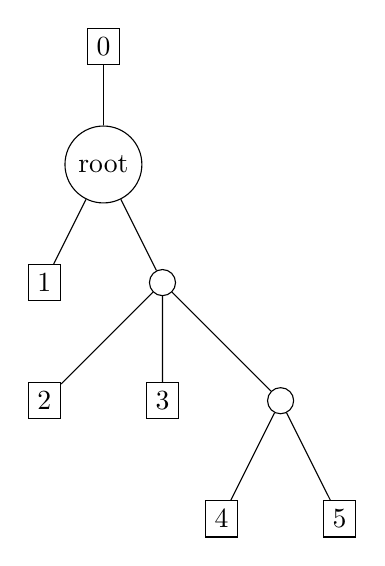
\begin{tikzpicture}
  \node[rectangle,draw] {0}
  child{node[circle,draw] {root}
      child {node[rectangle, draw, align=center] {1}}
      child {node[circle, draw] {}
        child {node[rectangle, draw, align=center] {2}}
        child {node[rectangle, draw, align=center] {3}}
        child {node[circle, draw] {}
          child {node[rectangle, draw, align=center] {4}}
          child {node[rectangle, draw, align=center] {5}}
        }
      }
    };
\end{tikzpicture}
\caption{Modified dimension tree $T_D$ with $d=5$ and special dimension 0}
\end{figure}

\subsection{Petrov-Galerkin projection}

The TT cross replaces the symmetric projection onto the solution interfaces by a Petrov-Galerkin
projection to sparsify the local systems.
We describe the analogon for tree-based tensors.

\paragraph{Interior nodes}
Consider an interior node $\alpha$, i.e. $\# \alpha > 1$, with adjacent nodes $\beta \in N(\alpha)$.
The projections $A^{(<\alpha)}_\beta$ are the analogon to the left projection in the TT algorithm.
It is the partial projection for a subtree of the matrix onto the solution.
$A^{(<\alpha)}_\beta \in \R^{r_u \times r_u \times r_A}$ is a tensor of dimension 3, with $r_u$ and $r_A$ being the rank between $\alpha$ and $\beta$ for the solution $\Bu$ and the matrix $\BA$ respectively.
Consequently, these differ for each $\alpha$ and $\beta$, but we omit this in the notation here.
We can give a recursive formula for $A^{(<\alpha)}_\beta$ using Einstein sum convention
\begin{equation}
  \label{eq:left_proj}
  A^{(<\alpha)}_\beta
  = \overline{\Bu^{(\alpha)}}[(j_k^{\overline{\Bu}})_{k \in K}] \
  \Bu^{(\alpha)}[(j_k^{\Bu})_{k \in K}] \
  \BA^{(\alpha)}[(j_k^{\BA})_{k \in K}] \
  \prod_{\gamma \in N(\alpha) \setminus {\beta}} A^{(<\alpha)}_\gamma[j_{k(\beta)}^{\overline{\Bu}} j_{k(\beta)}^{\Bu} j_{k(\beta)}^{\BA}]
\end{equation}
Here $K$ is an index set for the neighbours $N(\alpha)$, and $k(\beta)$ is the index associated with the neighbour $\beta$.

The projections $A^{(>\alpha)}_\beta$ correspond to the right projections.
In order to sparsify the projection, we choose maxvol indices $\CI$ in the matrization
$C = \Bu^{(\alpha)}[..., j_{k(\beta)}]$, ensure $C[\CI, :] = I$ by replacing $C C[\CI,:]^{-1}$ and
set
\begin{equation}
  \label{eq:right_proj}
  \tilde{A}^{(<\alpha)}_\beta
  = \overline{\Bu^{(\alpha)}}[(j_k^{\overline{\Bu}})_{k \in K}] \
  \Bu^{(\alpha)}[(j_k^{\Bu})_{k \in K}] \
  \BE[(j_k^{\BA})_{k \in K}] \
  \prod_{\gamma \in N(\alpha) \setminus {\beta}} A^{(<\alpha)}_\gamma[j_{k(\beta)}^{\overline{\Bu}} j_{k(\beta)}^{\Bu} j_{k(\beta)}^{\BA}]
\end{equation}
with $\BE[:, \dots, :, \CI, :, \dots, : ] = I$ when indexed with $\CI$ along the $k(\beta)$-th dimension.
For $\beta \in S(\alpha)$ \eqref{eq:right_proj} reduces by construction to
\begin{equation}
  \label{eq:right_proj}
  A^{(<\alpha)}_\beta
  = 
  \BA[(j_k^{\BA})_{k \in K \setminus \{k(\beta)\}}, j_{k(\beta)}^{\BA}][\CI, \colon] \
  \prod_{\gamma \in N(\alpha) \setminus {\beta}} A^{(<\alpha)}_\gamma[j_{k(\beta)}^{\overline{\Bu}} j_{k(\beta)}^{\Bu} j_{k(\beta)}^{\BA}]
\end{equation}
which are simply the (partial) subtree evaluations of $\BA$ at the nested maxvol indices.





\begin{algorithm}
\caption{ALS-cross algorithm for tree based tensors}


\begin{algorithmic}[1]
\Require{ Parameter as tree-based tensor, black-box solver $f$ to solve the linear system at parameter arbitrary indices, iteration count $n_{iter}$}
\Ensure{Tree-based tensor $\Bu$ approximating solution of parametric linear system}

\State Initialize:
\State Orthogonalize parameter tensors towards root and compute partial evals UA, Ub
\State random init solution tensor u
\State Init right hand projections of system UAU, UF
\State $i = 1$
\Repeat
  \State $U_0 \leftarrow f(I^{(\{0\})})$
  \Comment{solve at maxvol indices}
  \State $Q, R \leftarrow$ \Call{svd\_trunc}{$U_0$, $\varepsilon / \sqrt{d}$}
  \Comment{Orthogonalize and truncate}
  \State $\Bu^{(\{0\})} \leftarrow Q$
  \Comment{Update special core}
  \State $\Bu^{(D)}[\dots \widehat{j_p}] \leftarrow \Bu^{(D)}[\dots j_p] R[\widehat{j_p}, j_p]$
  \Comment{Cast non-orth factor to root node}
  \State Compute projections $(U^H A U)^{(\{0\})}$, $(U^H b)^{(\{0\})}$
  \Statex
  \State \Call{worker}{$D$}
  \Comment{Start DFS traversal at root}
  \State $i \leftarrow i + 1$
\Until{err $<$ tol or $i > n_{iter}$}
\Comment{Iterate}
\Statex
\Procedure{alsc\_worker}($\alpha$)
  \If{$\alpha$ is leaf}
    \State Solve reduced system
  \Else
    \State Solve reduced system
    \For{$\beta \in S(\alpha)$}
      \State $C[j_1 \dots j_{\# S(\alpha)} j_p , j_{i_c(\beta)}] 
        \leftarrow \Bv^{(\alpha)}[j_1 \dots j_{i_c(\beta)} \dots j_{\# S(\alpha)} j_p]$
      \Statex \Comment{Matrization with child index moved to the back}
      \State $Q, R \leftarrow$ \Call{svd\_trunc}{$C$, $\varepsilon / \sqrt{d}$}
      \Comment{Orthogonalize and truncate}
      \State $\Bu^{(\alpha)} \leftarrow Q$
      \Comment{update solution core}
      \State $ \Bv^{(\beta)}[j_1 \dots j_{\# S(\beta)} \widehat{j_p}]
      \leftarrow \Bv^{(\beta)} [j_1 \dots j_{\# S(\beta)} j_p] R[\widehat{j_{p}}, j_{p}]$
      \Statex \Comment{Cast non-orth factor to child; Einstein sum convention}
      \State update projections UAU and UF
      \State $R \leftarrow$ \Call{alsc\_worker}{$\beta$}
      \Comment{Recurse to child}
      \State $ \Bv^{(\alpha)}[j_1 \dots \widehat{j_{i_c(\beta)}} \dots j_{\# S(\alpha)} j_p]
      \leftarrow \Bv^{(\alpha)} [j_1 \dots j_{i_c(\beta)} \dots j_{\# S(\alpha)} j_p] R[\widehat{j_{i_c(\beta)}} j_{i_c(\beta)}]$
      \Statex \Comment{Absorb non-orth factor from child; Einstein sum convention}
    \EndFor
    \State Solve reduced system
    \State $C \leftarrow \Bv^{(\alpha)}[j_1 \dots j_{\# S(\alpha)}, j_p]$ \Comment{Matrization}
    \State $Q, R \leftarrow$ \Call{svd\_trunc}{$C$, $\varepsilon / \sqrt{d}$}
    \Comment{Orthogonalize and truncate}
    \State $I \leftarrow $ \Call{maxvol}{$Q$}
    \Comment{Compute maxvol indices}
    \State $\Bv^{(\alpha)} \leftarrow Q Q[I, :]^{-1}$
    \Comment{Set maxvol rows to identity}
    \State Update projections UA and Ub (sample param at indices)
    \State Update left interface projections UAU and UF
    \State return $Q[I, :] R$
    \Comment{Cast non-orth part to parent}

  \EndIf
\EndProcedure
\end{algorithmic}
\end{algorithm}

\newpage

\section{Appendix A: Utility procedures}

\begin{algorithm}
\caption{SVD based rank truncation - 2-norm}

\begin{algorithmic}[1]
\Procedure{svd\_trunc\_2}{$C$, $\varepsilon$}
\Comment{Truncate ranks of matrix $C \in \R^{m \times n}, m \geq n$ using SVD}
\State $U, S, V^H \leftarrow$ \Call{svd}{$C$}
\State $r \leftarrow \argmax_{j} s_j > s_1 \varepsilon$
\Comment{Truncation error bounded by $\varepsilon$ in 2-norm}
\State $ Q \leftarrow U[\colon, \colon r]$
\State $ R \leftarrow \operatorname{diag}(S[\colon r]) V^H[\colon r, \colon]$
\State return $Q,R$
\EndProcedure
\end{algorithmic}
\end{algorithm}

\begin{algorithm}
\caption{SVD based rank truncation - Frobenius norm}
\begin{algorithmic}[1]
\Procedure{svd\_trunc\_frob}{$C$, $\varepsilon$}
\Comment{Truncate ranks of matrix $C \in \R^{m \times n}, m \geq n$ using SVD}
\State $U, S, V^H \leftarrow$ \Call{svd}{$C$}
\State $r \leftarrow \argmax_{j} \sum_{i>j} s_i^2 > s_1^2 \varepsilon^2 $
\Comment{Truncation error bounded by $\varepsilon$ in Frobenius norm}
\State $ Q \leftarrow U[\colon, \colon r]$
\State $ R \leftarrow \operatorname{diag}(S[\colon r]) V^H[\colon r, \colon]$
\State return $Q,R$
\EndProcedure
\end{algorithmic}
\end{algorithm}

\begin{algorithm}
\caption{Rounding for tree-based tensors}
\begin{algorithmic}[1]
\Require{Tree-based tensor $\Bv$, tolerance $\varepsilon$}
\Ensure{Tree-based tensor $\Bv$ of reduced ranks}
\Call(worker\_trunc)

\Procedure{rounding\_worker}{$\alpha$}
\If{$\# \alpha = 1$}
\Comment{leaf}
\State $C \leftarrow \Bv^{(\alpha)}$
\State $Q, R \leftarrow$ \Call{svd\_trunc}{$C$, $\varepsilon / \sqrt{d}$}
\State $ \Bv^{(\alpha)} \leftarrow Q$
\State return $R$
\Comment{orthogonalize and truncate}
\Else
\Comment{interior node}
  \For{$\beta \in S(\alpha)$}
    \State $C[j_1 \dots j_{\# S(\alpha)} j_p , j_{i_c(\beta)}] 
      \leftarrow \Bv^{(\alpha)}[j_1 \dots j_{i_c(\beta)} \dots j_{\# S(\alpha)} j_p]$
      \Statex \Comment{Matrization with child index moved to the back}
      \State $Q, R \leftarrow$ \Call{svd\_trunc}{$C$, $\varepsilon / \sqrt{d}$}
      \Comment{Orthogonalize and truncate}
      \State $ \Bv^{(\beta)}[j_1 \dots j_{\# S(\beta)} \widehat{j_p}]
      \leftarrow \Bv^{(\beta)} [j_1 \dots j_{\# S(\beta)} j_p] R[\widehat{j_{p}}, j_{p}]$
      \Statex \Comment{Cast non-orth factor to child; Einstein sum convention}
      \State $R  \leftarrow $ \Call{rounding\_worker}{$\beta$}
      \Comment{recurse to child}
      \State $ \Bv^{(\alpha)}[j_1 \dots \widehat{j_{i_c(\beta)}} \dots j_{\# S(\alpha)} j_p]
      \leftarrow \Bv^{(\alpha)} [j_1 \dots j_{i_c(\beta)} \dots j_{\# S(\alpha)} j_p] R[\widehat{j_{i_c(\beta)}} j_{i_c(\beta)}]$
      \Statex \Comment{Absorb non-orth factor from child; Einstein sum convention}
  \EndFor

  \If{$\alpha \neq D$}
  \Comment{Skip for root}
    \State $C \leftarrow \Bv^{(\alpha)}[j_1 \dots j_{\# S(\alpha)},  j_p]$
    \Comment{Matrization}
      \State $Q, R \leftarrow$ \Call{svd\_trunc}{$C$, $\varepsilon / \sqrt{d}$}
      \Comment{Orthogonalize and truncate}
      \State $\Bv^{(\alpha)} \leftarrow Q$
      \State return $R$
  \EndIf
\EndIf
\EndProcedure
\end{algorithmic}
\end{algorithm}



\end{document}